%===========================================================================%
% 仲恺农业工程学院学位论文LaTeX模板
%===========================================================================%
%% ZHKU_Thesis.tex
%% Copyright 2024 Xinyu Ding <ding.xin.yu@foxmail.com> 
%
% This work may be distributed and/or modified under the
% conditions of the LaTeX Project Public License, either version 1.3
% of this license or (at your option) any later version.
% The latest version of this license is in
%   https://www.latex-project.org/lppl.txt
% and version 1.3c or later is part of all distributions of LaTeX
% version 2008 or later.
%===========================================================================%
%->> 文档类声明 Document class declaration
%---------------------------------------------------------------------------%
\documentclass[twoside]{Config/zhkuThesis}
%===========================================================================%
%->> 文档设置 Document settings
%---------------------------------------------------------------------------%
\usepackage[<super>, authoryear, list, table, math]{Style/artratex}
\usepackage{Style/artracom}
%===========================================================================%
%->> 文档包含 Document inclusion
%---------------------------------------------------------------------------%
%\includeonly{Tex/Chap_1,...,Tex/Chap_N}% selected files compilation
%===========================================================================%
%->> 文档内容 Document content
%===========================================================================%
%-
%-> 封面页信息 Titlepage information
%-
%---------------------------------------------------------------------------%
%->> 封面信息 Titlepage information
%---------------------------------------------------------------------------%
%-
%-> 中文封面信息
%-
\schoolCode{11347}
\studentCode{2112907013}
\classificationCode{S47 6}	
\confidential{} 
\schoolLogo[scale=1.2]{zhku_logo}
\title{东洋区冠果蝇亚科系统分类学研究(双翅目:果蝇科)}
\enTitle{Taxonomic Studies on the Subfamily Drosophila \\ (Diptera: Drosophilidae)}
\coverTitle{东洋区冠果蝇亚科系统分类学研究\\(双翅目:果蝇科)}
\authorName{高~~某}
\advisor{陈某某~~教授}
\institute{农业与生物学院}
\major{农业昆虫与害虫防治}
\city{中国·广州}
\degreeConferralDate{2024}{6}
%-
%-> 英文封面信息
%-
% TODO
%---------------------------------------------------------------------------%


\begin{document}

  % 无空白页 
  % 打开 \noblankpages 代码则输出不留空白页的PDF文件,适用于电子版传阅(如盲审)
  % 若取消这行代码(注释掉)则输出非正文部分重要页面从偶数页(右侧)开始的PDF文件,适用于打印出版
  \noblankpages

  % 盲审模式,打开则会使用“**”隐藏作者与导师相关相关信息,但是正文部分出现的个人信息则需要手动隐藏
  % \review

  % 学位类型:academic | professional
  % academic为学硕,professional为专硕,默认专硕
  \degreeType[professional]

  %-
  %-> 前置部分:封面、声明、摘要、目录列表、符号列表
  %-> Frontmatter: Title page, Declaration , Abstract, Content list, Symbol list
  %-
  \frontmatter{
    %---------------------------------------------------------------------------%
%->> 前言部分事项 Frontmatter
%---------------------------------------------------------------------------%
%-
%-> 生成封面
%-
\intobmk*{\cleardoublepage}{\coverNameMark~\titleMark}
% 生成中文封面
\pagecolor{orange}
\schoolLogo[height=2.2cm]{zhku_logo_gray}
\makeTitle
\pagecolor{white}
\schoolLogo[height=2.2cm]{zhku_logo}
\makeTitle
% TODO 生成英文封面
% \MAKETITLE

%-
%-> 书脊
%-
% 生成书脊页
\makespine

%-
%-> 作者声明
%-
% 生成声明页
\makeDeclaration

%-
%-> 中文摘要
%-
% 显示在书签但不显示在目录
\intobmk*{\cleardoublepage}{\abstractNameMark}
\begin{center}
    \heiti\bfseries\zihao{-3}\abstractName
    \thispagestyle{plain}
\end{center}

中文摘要、英文摘要、目录、论文正文、参考文献、附录、致谢、攻读学位期间发表的学术论文与其他相关学术成果等均须由另页右页(奇数页)开始。

摘要是论文的缩影,语言力求精炼准确。应概括论文的主要信息,包括研究目的、内容、结果和结论,要重点突出论文的新见解或创新性。硕士论文摘要字数800字左右。

关键词采用能覆盖论文主要内容的通用技术词条作为关键词,一般3至5个,按涉及的内容、领域从大到小排在摘要下方。

英文摘要内容与中文摘要基本一致,写作力求符合科技英语文法要求,英文摘要由论文题目、作者、作者单位、正文、关键词组成。


\keywords{仲恺农业工程学院;学位论文;Latex模板}% 中文关键词

%-
%-> 英文摘要
%-
\intobmk*{\cleardoublepage}{\enAbstractNameMark}
\begin{center}
    \heiti\bfseries\zihao{-3}\enTitleValue
    \thispagestyle{plain}
\end{center}

{
    \vspace{\baselineskip}
    \noindent\bfseries{\enAbstractName}
}

Chinese abstracts, English abstracts, table of contents, the main contents, references, appendix, acknowledgments, author's resume and academic papers published during the degree study and other relevant academic achievements must start with another right page (odd-numbered page).

\KEYWORDS{Zhongkai University of Agriculture and Engineering; Thesis; LaTeX Template}% 英文关键词
%---------------------------------------------------------------------------%

    % 符号表显示在书签但不显示在目录 Add symbols list into bookmark
\intobmk*{\cleardoublepage}{\symbolsNameMark}
\begin{center}
  \heiti\bfseries\zihao{-3}\symbolsName
  \pagestyle{plain}
\end{center}

% 字符 Character
\section*{\characterName}
\nomenclatureitem[\textbf{Unit}]{\textbf{Symbol}}{\textbf{Description}}
\nomenclatureitem[$\Unit{m^{2} \cdot s^{-2} \cdot K^{-1}}$]{$R$}{the gas constant}
\nomenclatureitem[$\Unit{m^{2} \cdot s^{-2} \cdot K^{-1}}$]{$C_v$}{specific heat capacity at constant volume}
\nomenclatureitem[$\Unit{m^{2} \cdot s^{-2} \cdot K^{-1}}$]{$C_p$}{specific heat capacity at constant pressure}
\nomenclatureitem[$\Unit{m^{2} \cdot s^{-2}}$]{$E$}{specific total energy}
\nomenclatureitem[$\Unit{m^{2} \cdot s^{-2}}$]{$e$}{specific internal energy}
\nomenclatureitem[$\Unit{m^{2} \cdot s^{-2}}$]{$h_T$}{specific total enthalpy}
\nomenclatureitem[$\Unit{m^{2} \cdot s^{-2}}$]{$h$}{specific enthalpy}
\nomenclatureitem[$\Unit{kg \cdot m \cdot s^{-3} \cdot K^{-1}}$]{$k$}{thermal conductivity}
\nomenclatureitem[$\Unit{kg \cdot m^{-1} \cdot s^{-2}}$]{$S_{ij}$}{deviatoric stress tensor}
\nomenclatureitem[$\Unit{kg \cdot m^{-1} \cdot s^{-2}}$]{$\tau_{ij}$}{viscous stress tensor}
\nomenclatureitem[$\Unit{1}$]{$\delta_{ij}$}{Kronecker tensor}
\nomenclatureitem[$\Unit{1}$]{$I_{ij}$}{identity tensor}

% 算子 Operator
\section*{\operatorName}
\nomenclatureitem{\textbf{Symbol}}{\textbf{Description}}
\nomenclatureitem{$\Delta$}{difference}
\nomenclatureitem{$\nabla$}{gradient operator}
\nomenclatureitem{$\delta^{\pm}$}{upwind-biased interpolation scheme}

% 缩写 Abbreviation
\section*{\abbreviationName}
\nomenclatureitem{CFD}{Computational Fluid Dynamics}
\nomenclatureitem{CFL}{Courant-Friedrichs-Lewy}
\nomenclatureitem{EOS}{Equation of State}
\nomenclatureitem{JWL}{Jones-Wilkins-Lee}
\nomenclatureitem{WENO}{Weighted Essentially Non-oscillatory}
\nomenclatureitem{ZND}{Zel'dovich-von Neumann-Doering}

\cleardoublepage

    \setcounter{page}{1}\pagenumbering{roman}
\pagestyle{noheaderstyle}

{
  % 将正文目录加入书签 Add into bookmark
  \intobmk*{\cleardoublepage}{\contentsNameMark}
  % 正文目录 Content catalog
  \tableofcontents\thispagestyle{noheaderstyle}
}


{
  % 将图标目录加入书签 Add into bookmark
  \intobmk*{\cleardoublepage}{\listFigureTableNameMark}

  \let\cleardoublepage\relax
  \let\clearpage\relax
  \renewcommand*{\addvspace}[1]{}
  \let\oldnumberline\numberline
  
  % 图目录 List of figures
  \renewcommand{\numberline}{\figurename~\oldnumberline}
  \listoffigures\thispagestyle{noheaderstyle}

  \renewcommand*{\addvspace}[1]{}
  \vspace{1cm}

  % 表目录 List of tables
  \renewcommand{\numberline}{\tablename~\oldnumberline}
  \listoftables\thispagestyle{noheaderstyle}
}


  }

  %-
  %-> 主体部分:正文、参考文献(不编号)
  %-> Mainmatter: Main text, Bibliography
  %-
  \mainmatter{
    \setlength{\parskip}{0.15\baselineskip}
    %---------------------------------------------------------------------------%
%->> Main content
%---------------------------------------------------------------------------%
% 开始页码
\setcounter{page}{1}
\thispagestyle{mainmatterstyle}

\chapter{绪论}\label{chap:introduction}
% \thispagestyle{noheaderstyle}

\section{背景}

2023年12月修订的《仲恺农业工程学院研究生学位论文撰写规范》(以下简称《规范》)从2024年1月1日开始实施。为方便各位同学使用,特提供此模板,该模板基于中国科学院大学研究生学位论文模板修改。

您在使用此模板进行学位论文撰写时,只需根据《规范》在相应章节填写具体内容即可。

本模板在第2章提供了本模板的使用说明,在第3章中提供了《规范》中关于内容和格式的部分要求,请仔细阅读。


\section{系统要求}\label{sec:system}
\begin{table}
    % 引用 caption
    \bicaption{\quad 支持的LaTeX编译系统和编辑器}{\quad Supported LaTeX compiler and editor}
    % 字体大小为脚注字体字号大小 set font size:foot font size
    \footnotesize
    % 设置表格列间距 column separation
    \setlength{\tabcolsep}{4pt}
    % 设置表格行高倍数 row space 
    \renewcommand{\arraystretch}{1.5}
    \centering
    \begin{tabular}{lcc}
        \Xhline{3\arrayrulewidth} % 加倍的宽度
        %\multicolumn{num_of_cols_to_merge}{alignment}{contents} \\
        %\cline{i-j}% partial hline from column i to column j
        操作系统 & LaTeX编译系统 & LaTeX文本编辑器\\
        \hline
        Windows & \href{https://www.tug.org/texlive/acquire-netinstall.html}{TexLive Full} 或 \href{https://miktex.org/download}{MiKTex} & \href{http://www.xm1math.net/texmaker/}{Texmaker}\\
        Linux & \href{https://www.tug.org/texlive/acquire-netinstall.html}{TexLive Full} & \href{http://www.xm1math.net/texmaker/}{Texmaker} 或 Vim\\
        MacOS & \href{https://www.tug.org/mactex/}{MacTex Full} & \href{http://www.xm1math.net/texmaker/}{Texmaker} 或 Texshop\\
        Overleaf & XeLaTeX+TexLive2021 & Overleaf \\
        \Xhline{3\arrayrulewidth} % 加倍的宽度
    \end{tabular}
    \label{tab:compiler}
\end{table}
\href{https://github.com/mohuangrui/ucasthesis}{\texttt{ucasthesis}} 宏包可以在目前主流的 \href{https://en.wikibooks.org/wiki/LaTeX/Introduction}{LaTeX} 编译系统中使用,如TexLive和MiKTeX。因CTex套装已停止维护,\textbf{不再建议使用} (请勿混淆CTex套装与ctex宏包。CTex套装是集成了许多LaTeX组件的LaTeX编译系统。 \href{https://ctan.org/pkg/ctex?lang=en}{ctex} 宏包如同ucasthesis,是LaTeX命令集,其维护状态活跃,并被主流的LaTeX编译系统默认集成,是几乎所有LaTeX中文文档的核心架构)。推荐的 \href{https://en.wikibooks.org/wiki/LaTeX/Installation}{LaTeX编译系统} 和 \href{https://en.wikibooks.org/wiki/LaTeX/Installation}{LaTeX文本编辑器} 为LaTeX编译系统见表~\ref{tab:compiler}。请从各软件官网下载安装程序,勿使用不明程序源。LaTeX编译系统和LaTeX编辑器分别安装成功后,即完成了LaTeX的系统配置,无需其他手动干预和配置。若系统原带有旧版的LaTeX编译系统并想安装新版,请\textbf{先卸载干净旧版再安装新版}。

使用overleaf在线编辑是一种简单有效的方法,对于绝大多数初学者来说,我们推荐使用这种无需进行系统配置的方式。在操作时,只需将压缩包上传至网站即可,无需在本地配置环境,同时支持多人,多地撰写论文。

本模板兼容操作系统:Windows、Linux、MacOS、Overleaf在线编辑器,支持多种LaTeX编译引擎(pdfLaTeX、xeLaTeX、luaLaTeX)。

\chapter{LaTeX使用说明}\label{chap:guide}
% \thispagestyle{noheaderstyle}

{
为方便使用及更好地展示LaTeX排版的优秀特性,ucasthesis的框架和文件体系进行了细致地处理,尽可能地对各个功能和板块进行了模块化和封装。zhkuThesis基于ucasthesis做了自定义的样式修改和整理说明。

\section{初步设置}

\begin{enumerate}
    \item 使用overleaf:打开并注册\href{https://cn.overleaf.com/}{overleaf}。
    \item 将整个文件夹上传至overleaf项目。
    \item 右键菜单,设置编译器为XeLaTeX,选择TexLive 2021
    \item 点击编译,即可预览PDF文件
\end{enumerate}

编译完成即可获得本PDF说明文档。

\section{文档目录简介}

\subsection{zhkuThesis.tex}

zhkuThesis.tex为主文档,其设计和规划了论文的整体框架,通过对其的阅读可以了解整个论文框架的搭建。

\subsection{编译脚本}

为方便本地编译,提供bat脚本和.sh脚本分别用于windows环境和unix环境。

\begin{itemize}
    \item Windows:双击Dos脚本artratex.bat可得全编译后的PDF文档,其存在是为了帮助不了解LaTeX编译过程的初学者跨过编译这第一道坎,请勿通过邮件传播和接收此脚本,以防范Dos脚本的潜在风险。
    \item Linux或MacOS:在terminal中运行
        \begin{itemize}
            \item \verb|./artratex.sh xa|:获得全编译后的PDF文档
            \item \verb|./artratex.sh x|:快速编译,不会生成文献引用
        \end{itemize}
\end{itemize}

全编译指运行 \verb|xeLaTeX+bibtex+xeLaTeX+xeLaTeX| 以正确生成所有的引用链接,如目录、参考文献及引用等。在写作过程中若无添加新的引用,则可用快速编译,即只运行一遍LaTeX编译引擎以减少编译时间。

\subsection{Tmp文件夹}

运行编译脚本后,编译所生成的文档皆存于Tmp文件夹内,包括编译得到的PDF文档,其存在是为了保持工作空间的整洁。

\subsection{Style文件夹}

包含zhkuThesis文档类的定义文件和配置文件,通过对它们的修改可以实现特定的模版设定。

\begin{enumerate}
    \item zhkuThesis.cls:文档类定义文件,论文的最核心的格式即通过它来定义的。
    \item zhkuThesis.cfg:文档类配置文件,设定如目录显示为“目~录”而非“目录”。
    \item artratex.sty: 常用宏包及文档设定,如参考文献样式、文献引用样式、页眉页脚设定等。这些功能具有开关选项,常只需在Thesis.tex中进行启用即可,一般无需修改artratex.sty本身。
    \item artracom.sty:自定义命令以及添加宏包的推荐放置位置。
\end{enumerate}

\subsection{Tex文件夹}

文件夹内为论文的所有实体内容,正常情况下,这也是使用zhkuThesis撰写学位论文时,主要关注和修改的一个位置,注:所有文件都必须采用UTF-8编码,否则编译后将出现乱码文本,详细分类介绍如下:

\begin{itemize}
    \item Frontinfo.tex:为论文中英文封面信息。论文封面会根据英文学位名称如Master,Doctor自动切换为相应的格式。
    \item Frontmatter.tex:为论文前言内容如中英文摘要等。
    \item Mainmatter.tex:索引需要出现的Chapter。开始写论文时,可以只索引当前章节,以快速编译查看,当论文完成后,再对所有章节进行索引即可。
    \item Chap{\_}xxx.tex:为论文主体的各章,可根据需要添加和撰写。添加新章时,可拷贝一个已有的章文件再重命名,以继承文档的 UTF8 编码。
    \item Appendix.tex:为附录内容。
    \item Backmatter.tex:为发表文章信息和致谢部分等。
\end{itemize}

\subsection{Image文件夹}

用于放置论文中所需要的图类文件,支持格式有:.jpg, .png, .pdf。其中,\verb|zhku_logo.png|为仲恺农业工程学院校徽校名。

\subsection{Biblio文件夹}

 ref.bib用于放置论文中所需要参考文献信息。

\section{功能介绍}

\subsection{数学公式}

比如Navier-Stokes方程(方程~\eqref{eq:ns}):
\begin{equation} \label{eq:ns}
    %\adddotsbeforeeqnnum%
    \begin{cases}
        \frac{\partial \rho}{\partial t} + \nabla\cdot(\rho\Vector{V}) = 0 \ \mathrm{times\ math\ test: 1,2,3,4,5}, 1,2,3,4,5\\
        \frac{\partial (\rho\Vector{V})}{\partial t} + \nabla\cdot(\rho\Vector{V}\Vector{V}) = \nabla\cdot\Tensor{\sigma} \ \text{times text test: 1,2,3,4,5}\\
        \frac{\partial (\rho E)}{\partial t} + \nabla\cdot(\rho E\Vector{V}) = \nabla\cdot(k\nabla T) + \nabla\cdot(\Tensor{\sigma}\cdot\Vector{V})
    \end{cases}
\end{equation}
\begin{equation}
    %\adddotsbeforeeqnnum%
    \frac{\partial }{\partial t}\int\limits_{\Omega} u \, \mathrm{d}\Omega + \int\limits_{S} \unitVector{n}\cdot(u\Vector{V}) \, \mathrm{d}S = \dot{\phi}
\end{equation}
\[
    \begin{split}
        \mathcal{L} \{f\}(s) &= \int _{0^{-}}^{\infty} f(t) e^{-st} \, \mathrm{d}t, \ 
        \mathscr{L} \{f\}(s) = \int _{0^{-}}^{\infty} f(t) e^{-st} \, \mathrm{d}t\\
        \mathcal{F} {\bigl (} f(x+x_{0}) {\bigr )} &= \mathcal{F} {\bigl (} f(x) {\bigr )} e^{2\pi i\xi x_{0}}, \ 
        \mathscr{F} {\bigl (} f(x+x_{0}) {\bigr )} = \mathscr{F} {\bigl (} f(x) {\bigr )} e^{2\pi i\xi x_{0}}
    \end{split}
\]

数学公式常用命令请见 \href{https://en.wikibooks.org/wiki/LaTeX/Mathematics}{WiKibook Mathematics}。artracom.sty中对一些常用数据类型如矢量矩阵等进行了封装,这样的好处是如有一天需要修改矢量的显示形式,只需单独修改artracom.sty中的矢量定义即可实现全文档的修改。

\subsection{数学环境}

\begin{axiom}
   这是一个公理。 
\end{axiom}
\begin{theorem}
   这是一个定理。 
\end{theorem}
\begin{lemma}
   这是一个引理。 
\end{lemma}
\begin{corollary}
   这是一个推论。 
\end{corollary}
\begin{assertion}
   这是一个断言。 
\end{assertion}
\begin{proposition}
   这是一个命题。 
\end{proposition}
\begin{definition}
    这是一个定义。
\end{definition}
\begin{example}
    这是一个例子。
\end{example}
\begin{remark}
    这是一个注。
\end{remark}

\subsection{图}

论文中图片的插入通常分为单图和多图,下面分别加以介绍:

单图插入:假设插入名为\verb|c06h06|(后缀可以为.jpg、.png和.pdf,下同)的图片,其效果如图~\ref{fig:c06h06}。
\begin{figure}[!htbp]
    \centering
    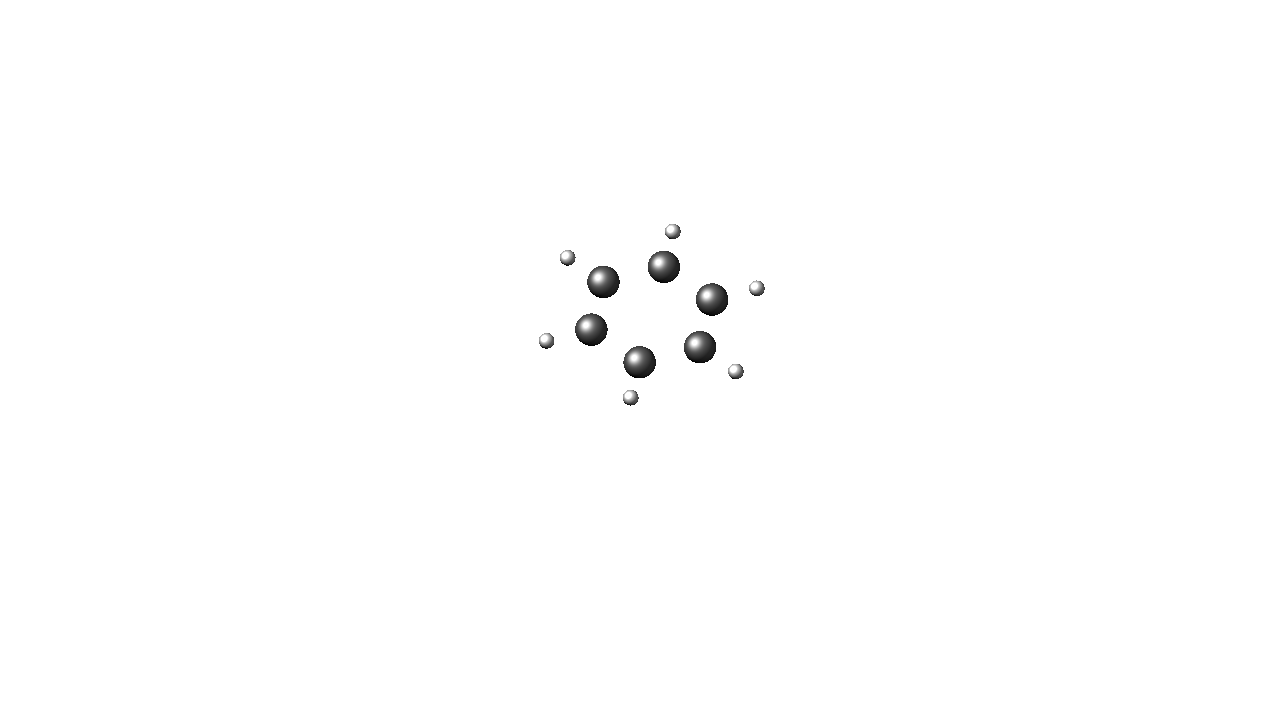
\includegraphics[width=0.40\textwidth]{c06h06}
    \bicaption{\quad 样图}{\quad Sample Figure}
    \label{fig:c06h06}
\end{figure}

如果插图的空白区域过大,以图片\verb|c06h06|为例,自动裁剪如图~\ref{fig:c06h06_trim}。
\begin{figure}[!htbp]
    \centering
    %trim option's parameter order: left bottom right top
    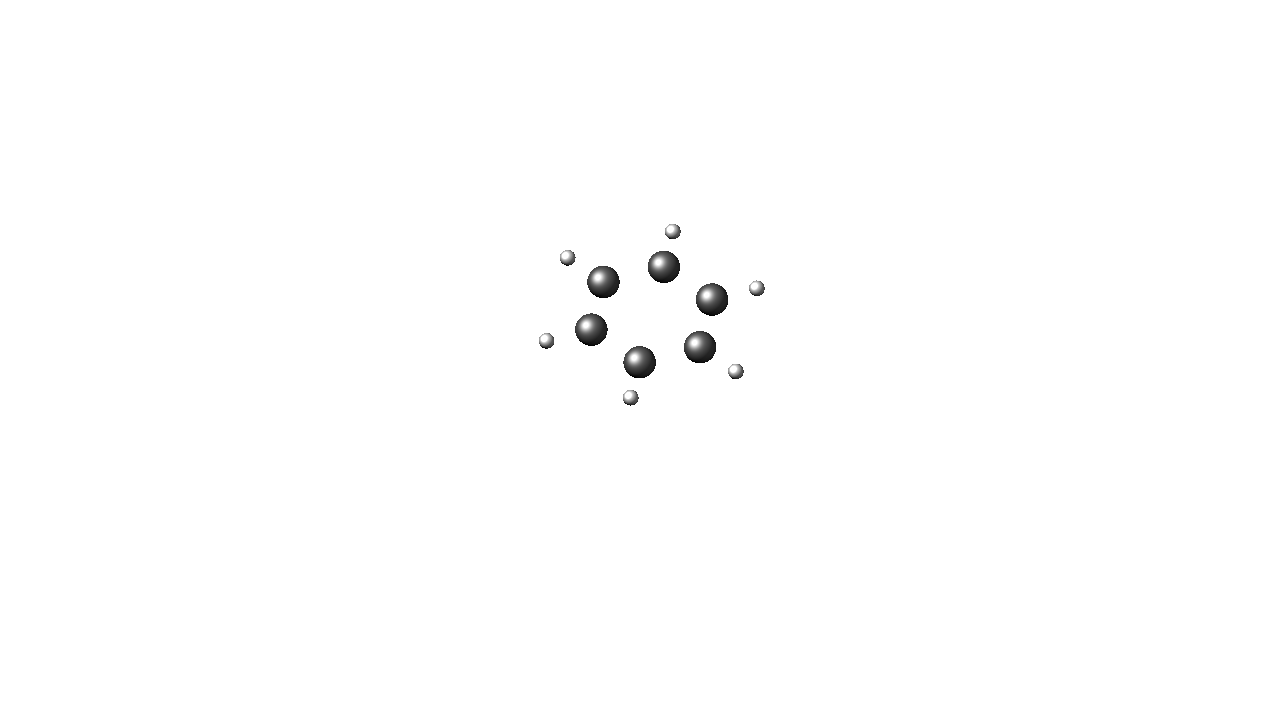
\includegraphics[trim = 60mm 80mm 60mm 60mm, clip, width=0.40\textwidth]{c06h06}
    \bicaption{\quad 自动裁切测试}{\quad Auto-Crop Test}
    \label{fig:c06h06_trim}
\end{figure}

多图的插入如图~\ref{fig:oaspl},多图不应在子图中给文本子标题,只要给序号,并在主标题中进行引用说明。
\begin{figure}[!htbp]
    \centering
    \begin{subfigure}[b]{0.35\textwidth}
      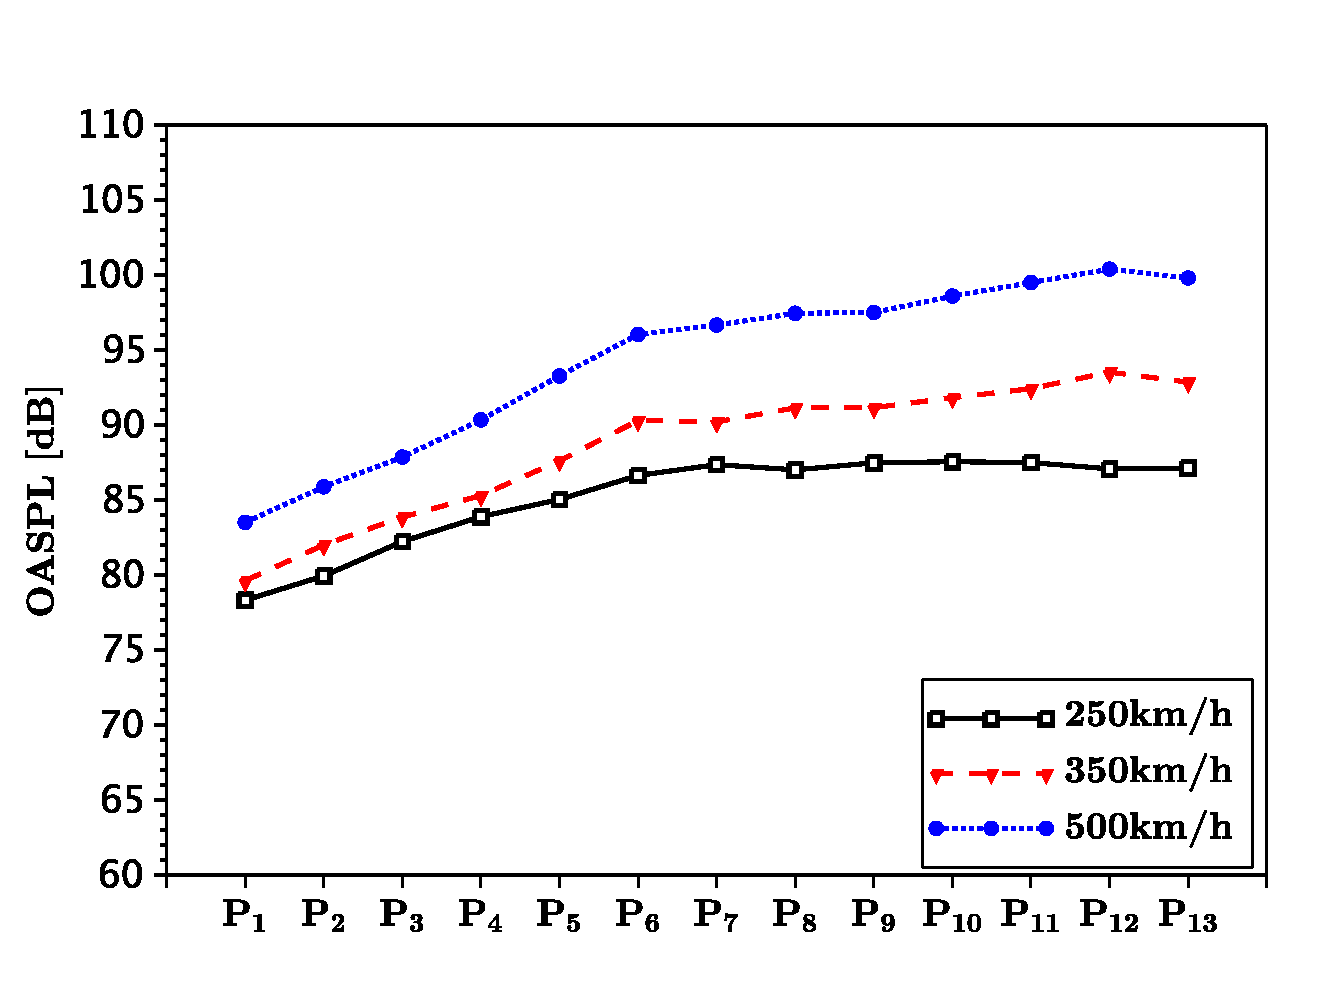
\includegraphics[width=\textwidth]{oaspl_a}
      \caption{}
      \label{fig:oaspl_a}
    \end{subfigure}%
    ~% add desired spacing
    \begin{subfigure}[b]{0.35\textwidth}
      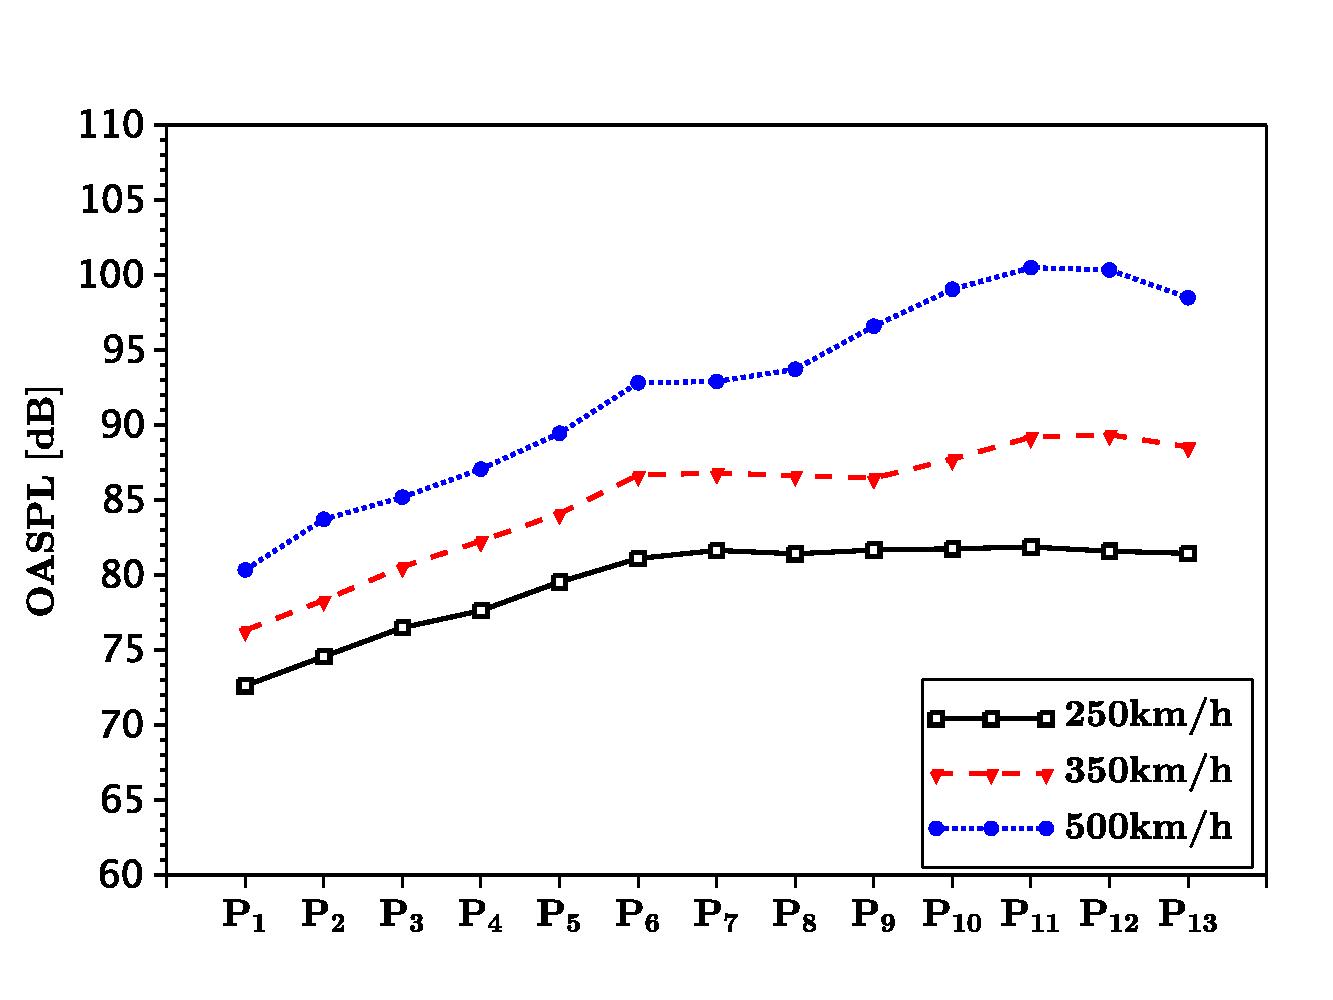
\includegraphics[width=\textwidth]{oaspl_b}
      \caption{}
      \label{fig:oaspl_b}
    \end{subfigure}
    \\% line break
    \begin{subfigure}[b]{0.35\textwidth}
      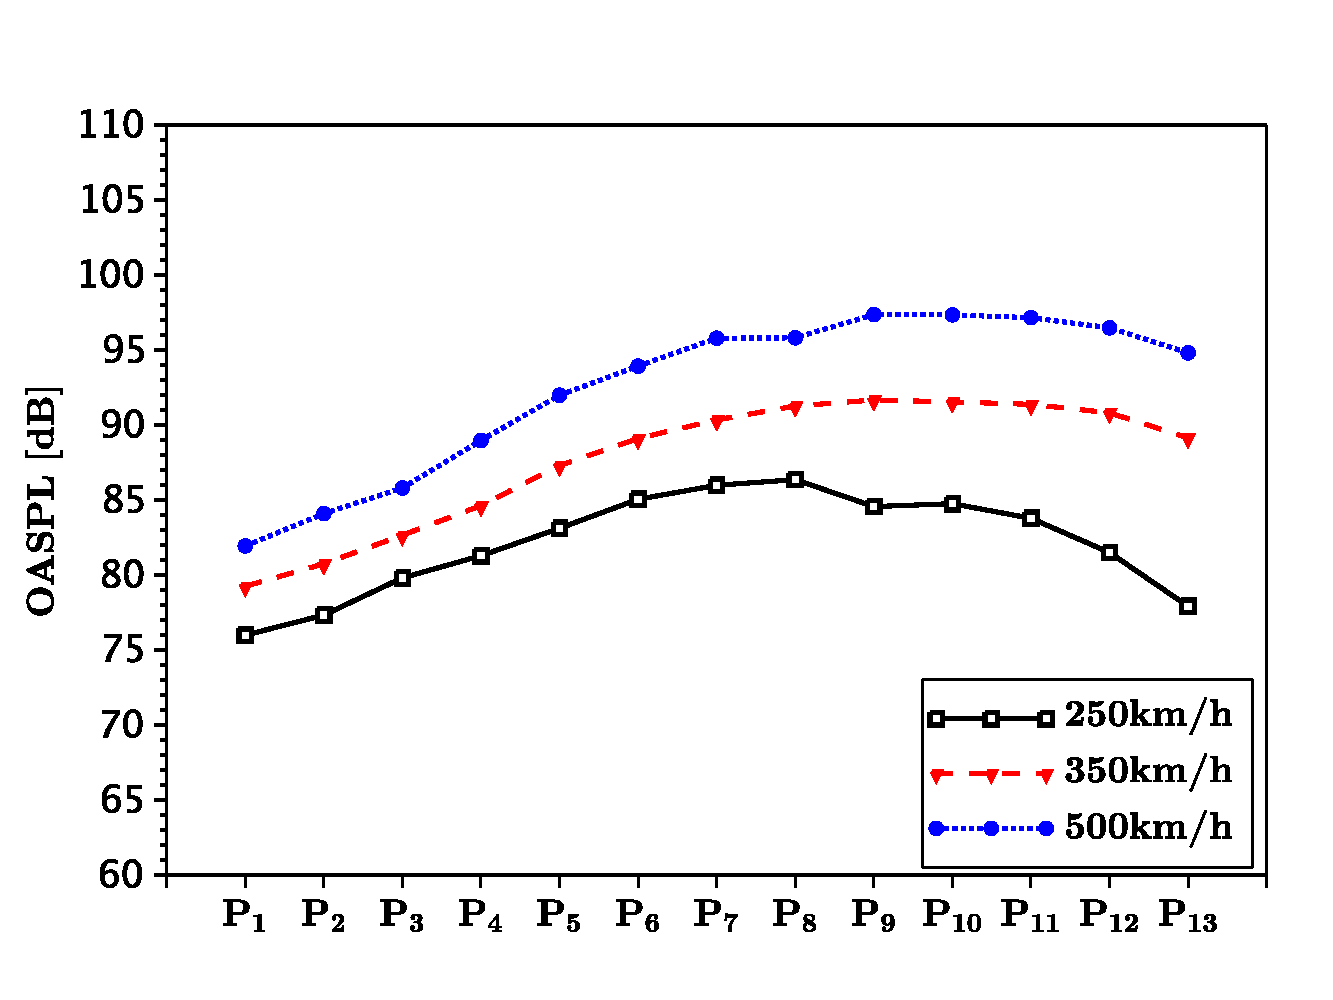
\includegraphics[width=\textwidth]{oaspl_c}
      \caption{}
      \label{fig:oaspl_c}
    \end{subfigure}%
    ~% add desired spacing
    \begin{subfigure}[b]{0.35\textwidth}
      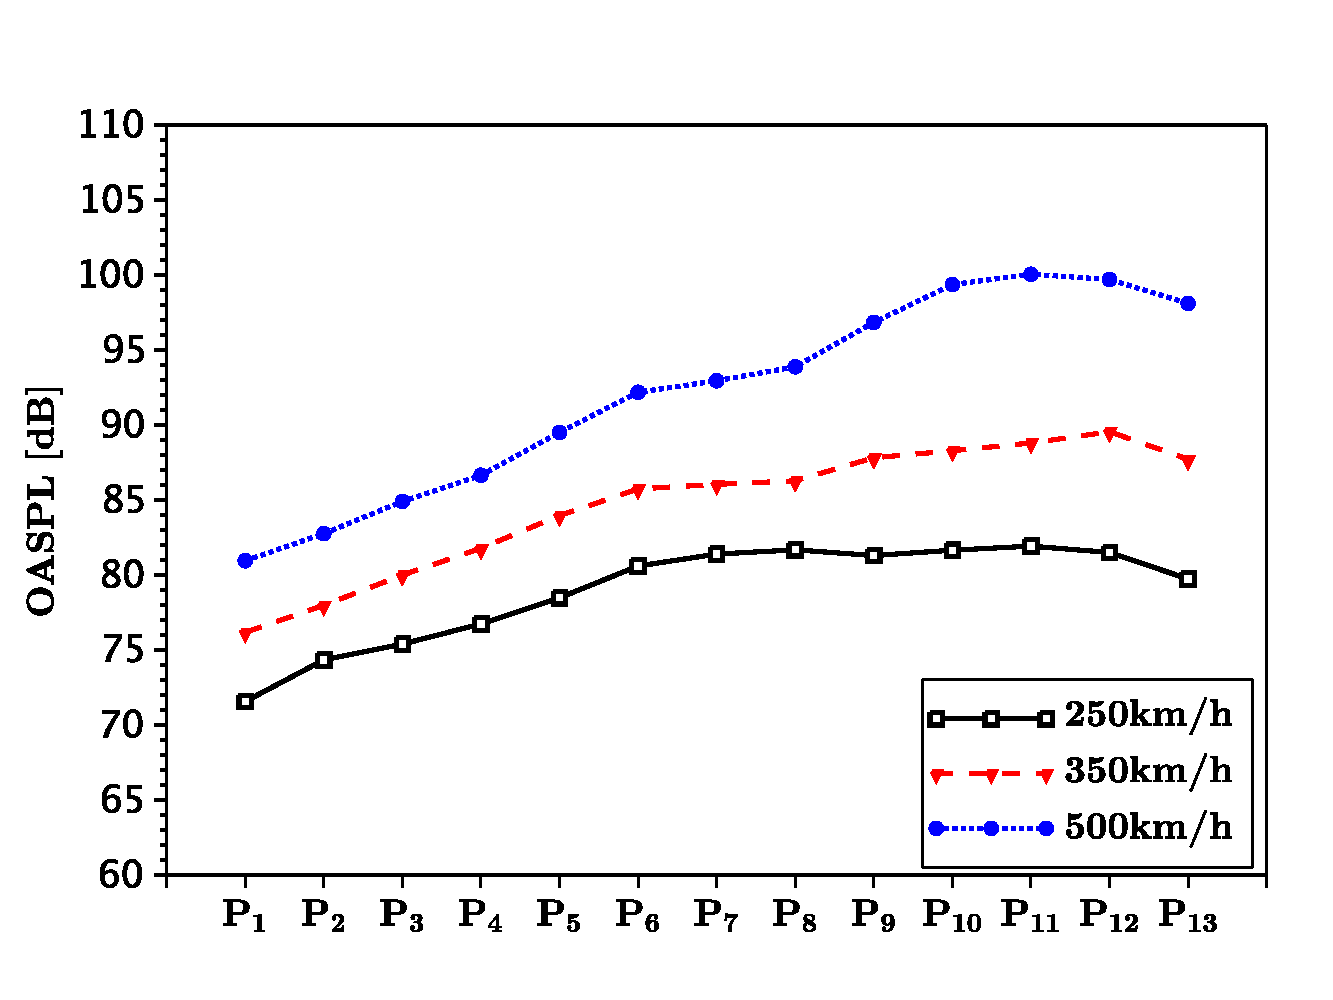
\includegraphics[width=\textwidth]{oaspl_d}
      \caption{}
      \label{fig:oaspl_d}
    \end{subfigure}
    \bicaption{\quad 多子图测试}{\quad A test for multi-subfig}
    \label{fig:oaspl}
\end{figure}

\subsection{表}

请见表~\ref{tab:sample}。
\begin{table}[!htbp]
    \bicaption{\quad 这是一个样表}{\quad This is a sample table}
    \label{tab:sample}
    \centering
    \footnotesize% fontsize
    \setlength{\tabcolsep}{4pt}% column separation
    \renewcommand{\arraystretch}{1.2}%row space 
    \begin{tabular}{lcccccccc}
        \Xhline{3\arrayrulewidth} % 加倍的宽度
        行号 & \multicolumn{8}{c}{跨多列的标题}\\
        %\cline{2-9}% partial hline from column i to column j
        \hline
        Row 1 & $1$ & $2$ & $3$ & $4$ & $5$ & $6$ & $7$ & $8$\\
        Row 2 & $1$ & $2$ & $3$ & $4$ & $5$ & $6$ & $7$ & $8$\\
        Row 3 & $1$ & $2$ & $3$ & $4$ & $5$ & $6$ & $7$ & $8$\\
        Row 4 & $1$ & $2$ & $3$ & $4$ & $5$ & $6$ & $7$ & $8$\\
        \Xhline{3\arrayrulewidth} % 加倍的宽度
    \end{tabular}
\end{table}

制图制表的更多范例,请见 \href{https://github.com/mohuangrui/ucasthesis/wiki}{ucasthesis 知识小站} 和 \href{https://en.wikibooks.org/wiki/LaTeX/Tables}{WiKibook Tables}。

\subsection{参考文献引用}

参考文献引用过程以实例进行介绍,假设需要引用名为"Document Preparation System"的文献,步骤如下:

1)将Bib格式的参考文献信息添加到ref.bib文件中(此文件位于Biblio文件夹下),如直接粘贴自网站,请注意修改其格式。

2)索引第一行 \verb|@article{lamport1986document,|中 \verb|lamport1986document| 即为此文献的label (中文文献也必须使用英文label,一般遵照:姓氏拼音+年份+标题第一字拼音的格式),想要在论文中索引此文献,\verb|\citep{lamport1986document}|。如此处所示 \citep{lamport1986document}。

多文献索引用英文逗号隔开, 如此处所示 \citep{lamport1986document, chu2004tushu, chen2005zhulu}。

更多例子如:

Walls等\citep{walls2013drought}根据Betts\citep{betts2005aging} 的研究,首次提出......理论。其中关于......的研究\citepns{walls2013drought, betts2005aging},是当前中国得到迅速发展的研究领域 \citep{chen1980zhongguo, bravo1990comparative}。

不同文献样式和引用样式,如著者-出版年制(authoryear)、顺序编码制(numbers)、上标顺序编码制(super)可在Thesis.tex中对artratex.sty调用实现,详见 \href{https://github.com/mohuangrui/ucasthesis/wiki}{ucasthesis 知识小站之文献样式}。

%若在上标顺序编码制(super)模式下,希望在特定位置将上标改为嵌入式标,可使用 \citetns{niu2013zonghe,stamerjohanns2009mathml} 和 \citepns{niu2013zonghe,stamerjohanns2009mathml}。

参考文献索引的更多知识,请见 \href{https://en.wikibooks.org/wiki/LaTeX/Bibliography_Management}{WiKibook Bibliography}。\nocite{*}% 使文献列表显示所有参考文献(包括未引用文献)

\section{常见使用问题}\label{sec:qa}

设置文档样式: 在artratex.sty中搜索关键字定位相应命令,然后修改
\begin{enumerate}
    \item 正文行距:启用和设置 \verb|\linespread{1.25}|,默认1.25倍行距。
    \item 参考文献行距:修改 \verb|\setlength{\bibsep}{0.0ex}|
    \item 目录显示级数:修改 \verb|\setcounter{tocdepth}{2}|
    \item 文档超链接的颜色及其显示:修改 \verb|\hypersetup|
\end{enumerate}

文档内字体切换方法:
    \begin{itemize}
        \item 宋体:国科大论文模板ucasthesis 或 \textrm{国科大论文模板ucasthesis}
        \item 粗宋体:{\bfseries 国科大论文模板ucasthesis} 或 \textbf{国科大论文模板ucasthesis}
        \item 黑体:{\sffamily 国科大论文模板ucasthesis} 或 \textsf{国科大论文模板ucasthesis}
        \item 粗黑体:{\bfseries\sffamily 国科大论文模板ucasthesis} 或 \textsf{\bfseries 国科大论文模板ucasthesis}
        \item 仿宋:{\ttfamily 国科大论文模板ucasthesis} 或 \texttt{国科大论文模板ucasthesis}
        \item 粗仿宋:{\bfseries\ttfamily 国科大论文模板ucasthesis} 或 \texttt{\bfseries 国科大论文模板ucasthesis}
        \item 楷体:{\itshape 国科大论文模板ucasthesis} 或 \textit{国科大论文模板ucasthesis}
        \item 粗楷体:{\bfseries\itshape 国科大论文模板ucasthesis} 或 \textit{\bfseries 国科大论文模板ucasthesis}
    \end{itemize}

\let\cleardoublepage\relax
}

\chapter[研究生学位论文撰写规范]{仲恺农业工程学院研究生学位论文撰写规范\\(2023年12月修订)}\footnotetext{来源:关于印发《仲恺农业工程学院研究生学位论文写作规范(2023年修订)》的通知 https://yjs.zhku.edu.cn/info/1060/4945.htm}
{
\let\cleardoublepage\relax
}

为进一步规范研究生学位论文撰写,提高学位论文质量,根据国家相关标准和我校实际情况,特制定如下规范:

\section{研究生学位论文结构}

学位论文基本结构包括前置部分、主体部分和附录部分。

\subsection{前置部分}

\begin{enumerate}
    \item 封面
    \item 原创性声明、版权使用授权书、学位论文提交同意书
    \item 中文摘要、英文摘要
    \item 英文缩略词或符号表
    \item 目录
\end{enumerate}

\subsection{主体部分}

\begin{enumerate}
    \item 正文
    \item 参考文献
\end{enumerate}

\subsection{附录部分}

\begin{enumerate}
    \item 不便列入正文的材料、数据等
    \item 攻读学位期间的研究成果、获奖情况和参研项目等
    \item 致谢
\end{enumerate}

\section{研究生学位论文写作要求}

\subsection{封面及书脊}

\begin{enumerate}
  \item 封面内容包括学校代码、分类号、密级、论文题目、学号、作者姓名、指导教师、学院、专业(领域)等。
  \item 分类号:注明《中国图书资料分类法》的类号。
  \item 密级:必须按国家规定的保密条例和学位论文开题前申请的密级填写,非涉密论文不能填写。涉密学位论文须在封面“密级”后标明密级和保密期限,标志符号为“★”,“★”前标密级,“★”后标保密期限,例如“秘密★5年”。
  \item 题目:学位论文题目要精炼,起画龙点睛的效果,字数一般不得超过26个字。
  \item 作者姓名:填写研究生姓名。
  \item 指导教师:所列出的指导教师必须是已在研究生部备案的指导教师。
  \item 学院:填申请学位所在学院。
  \item 专业(领域)名称:按国家颁布的学科、专业目录中的名称填写。
  \item 书脊内容包括学位论文题目、作者姓名、学校名称和年份。
\end{enumerate}

\subsection{原创性声明、版权使用授权书、学位论文提交同意书}

\begin{enumerate}
  \item 原创性声明:论文作者签名。
  \item 版权使用授权书:论文作者和导师签名。
  \item 学位论文提交同意书:导师审核学位论文并签名。
\end{enumerate}

\subsection{中文摘要}

摘要是论文的缩影,语言力求精炼准确。应概括论文的主要信息,包括研究目的、内容、结果和结论,要重点突出论文的新见解或创新性。硕士论文摘要字数800字左右。

关键词采用能覆盖论文主要内容的通用技术词条作为关键词,一般3至5个,按涉及的内容、领域从大到小排在摘要下方。

\subsection{英文摘要}

英文摘要内容与中文摘要基本一致,写作力求符合科技英语文法要求,英文摘要由论文题目、作者、作者单位、正文、关键词组成。

\subsection{英文缩略词或符号表}

如有英文缩略词或符号表,应放在英文摘要之后,目录之前。

\subsection{目录}

目录置于摘要之后。目录正文需列出论文各章节标题及页码。目录中各层次标题与正文层次标题一致。原创性声明、版权使用授权书、学位论文提交同意书、中文摘要、英文摘要不编入目录中。致谢、参考文献、附录一律不编序号。

\subsection{正文}

正文是学位论文的主体部分,论文内容必须立论正确、言之成理、论据可靠、阐述透彻、逻辑严密,论文书写要层次分明、思路清晰、文字简练、结构完整。正文撰写必须严格遵守学术规范,论文中如引用他人的论点或数据资料,必须注明出处,引用合作者的观点或研究成果时,要加注说明,否则将被视为剽窃行为。正文部分具体研究内容应是论文作者自己的研究成果,不能将他人研究成果不加区分地掺和进来。结论中要严格区分自己取得的成果与导师及他人的科研工作成果,评价研究工作成果时,要实事求是。

学位论文的研究主题切忌过大,通常只有一个主题(不能是几部分研究工作的简单拼凑),该主题应针对某学科领域中的一个具体问题展开深入、系统地研究,并得出有价值的研究结论。

\begin{enumerate}

    \item 正文结构
    
    由于学位论文研究工作涉及的学科专业特点、论文选题情况研究方法、工作进程、结果表达方式、学位论文形式等有很大的差异,学位论文正文结构有不同的写作方式。正文的撰写结构具体参考《研究生学位论文正文结构规范》。

    \item 各级标题
    
    正文层次标题应简短明确,以不超过15字为宜,题末不加标点符号。各层次一律用阿拉伯数字连续编号,(如“1”,“2.1”,“3.1.2”)一律左对齐,后空一个字符写标题。各级标题与段落之间不留空行。
    
    \item 图、表、公式
    
    (1)图、表力求简明,自明性强。图与表的内容不得重复,并尽可能紧随相应的文字描述排列。图、表一般不得分页排列,若无法避免,须在另一页制作独立表头。
    
    (2)表一般应该采用“三线式”,表格的上下边框线宽度为1.5磅,中线宽度为0.5磅。有分图时,分图用a、b、c表示。
    
    (3)图、表与正文之间须设置段前段后0.5行间距,图题、表题与图、表之间不留空行。
    
    (4)学位论文中的图题、表题应采用中英文对照,中文居上。
    
    (5)图题居图下方,表题居表上方,用阿拉伯数字编号,如:图1或图1.1(表1或表1.1),图号后空1个字符写图题。
    
    (6)论文若有多个公式,按章节采用(1.1)、(1.2)等编号方式,公式编号写在右边行末,其间不加虚线。
    
    \item 数据分析
    
    论文中试验数据的统计分析,如果是应用计算机软件的,尽可能采用公开发行的程序;如果是自编的,应在附录中列出程序。在数据分析中各试验数据的平均数之后应列出平均数的标准误(S.E.)。如列出标准误(S.D.)的要注明样本数n值。
    
    \item 注释
    
    注释是论文中的解释性说明词句,采用“脚注”方式,以右上标的形式在注释处标注序号(圆括号加数字),并在当前页下按序号顺序列出注释的内容。注释的序号每页单独排序。
    
    \item 量和单位
    
    应严格执行GB 3100-1993、GB/T 3101-1993、GB/T 3102.1~13-1993有关量和单位的规定(参阅《常用量和单位》.计量出版社,1996)。单位名称的书写,可采用国际通用符号,也可用中文名称,但全文应统一,不要两种混用。
    (1)文中所用的量度单位按“中国高等学校自然科学学报编排规范”(北京工业大学出版社,1993)中“附录B量和单位”的规定,如公斤用kg。但在正文叙述时,应用中文表述,如:“每克”,而不要用“每g”。
    (2)文中采用英文字母缩写的,第一次出现时应把英文的全称写出,如:Gross National Product(GNP)、Diamond Back Moth(DBM)。

\end{enumerate}

\subsection{参考文献}

参考文献格式基本遵守GB/T7714-2015《信息与文献——参考文献著录规则》,但主要有以下两点不同:

\begin{enumerate}
  \item 正文中的引文标注
  
  默认形式是“(作者,出版年)”。当文中已提到作者时,只需在括号中注明出版年,即“作者(出版年)”。若在同一处引用多篇参考文献,则改为“(作者,出版年;作者,出版年)”并按出版年份先后排序。
  
  \item 文后参考文献列表
  
  建议采用Note Express软件进行处理,先选用“中华人民共和国国家标准\_GBT\_7714-2015”样式,随后须进行手动修改。
  
  引文开头的序号、空格应删除;取消段落缩进,全选并点击右键,在“段落”选项内将“悬挂缩进”改为“无”。列表按作者姓名排序,中文文献在前,外文文献在后。(详见《学位论文中写作中使用Note Express处理文献引用指南》)
  
\end{enumerate}

\subsection{附录}

如有附录,应编入目录中。附录是正文主体的补充。攻读学位期间发表的(含已录用,并有录用通知书的)与学位论文相关的学术论文,由于篇幅过大或取材于复制件不便编入正文的材料、数据,对本专业同行有参考价值但对一般读者不必阅读的材料,论文所使用计算机程序清单、软磁盘,成果鉴定证书、获奖奖状或专利证书的复印件等可作为附录内容。有多项附录内容时,采用附录A、附录B等编号。

\subsection{致谢}

致谢中的用词和用语不要过于渲染。内容应简洁明了、实事求是。凡在读研究生不得称谓硕士。

\subsection{其他}

论文中的物理量名称、符号及计量单位一律采用国务院发布的《中华人民共和国法定计量单位》,单位名称和符号的书写方式,应采用国际通用符号。

除特殊需要外,全文用汉语简化字,英文数字用“Times New Roman”字体。

资助论文的科研项目可在“致谢”中标出。

学位论文要求用中文写作。外国留学生或与国际研究课题合作完成的论文可用英文撰写,但必须用中文撰写较详细的“摘要”。


\section{研究生学位论文格式要求}

\subsection{论文纸张要求}

采用A4纸(21cm×29.7cm)双面打印。封面纸质为180-200g/m²,硕士学位论文封面为橙色,其他部分用普通白色A4纸。

\subsection{页面设置}

\begin{enumerate}
  \item 边距:上、下边距2.5cm,左、右边距2.7cm,页眉1.5cm,页脚1.75cm。
  \item 行间距:1.5倍。
  \item 页码:页码居中。前置部分从中文摘要到目录的页码用大写罗马数字,主体部分用阿拉伯数字。
\end{enumerate}

\subsection{字体、字号与排版要求}

% FIXME 表格里面列表结束之后会有空一行
\begin{center}
  \begin{longtable}{m{5cm}m{9cm}}
    \bicaption{\quad 字体、字号与排版要求}{\quad Font, Size, Typography Requirements} \label{tab:printrequirements} \\
  
    \hline\hline \textbf{内容} & \textbf{格式要求} \\ \hline\hline
    \endfirsthead
    
    \multicolumn{2}{c}%
    {{\bfseries \tablename\ \thetable{} -- 续上表}} \\
    \hline\hline \multicolumn{1}{c}{\textbf{内容}} & \multicolumn{1}{c}{\textbf{格式要求}} \\ \hline\hline
    \endhead
    
    \hline \multicolumn{2}{r}{{接下表}} \\
    \endfoot
    
    \hline \hline
    \endlastfoot
    
    封面及书脊 & 要求按照示例模板。\\
    原创性声明、版权使用授权书、论文提交同意书 & 要求按照示例模板。\\
    中文摘要及关键词 & 
    \begin{enumerate}
      \item “摘要”两字居中,两字之间留空4个字符,四号黑体,摘要正文小四号宋体。
      \item “关键词”三个字小四号黑体,与摘要靠左对齐,后加“:”,关键词之间用分号隔开,小四号宋体。
    \end{enumerate}\\
    英文摘要及关键词 & 
    \begin{enumerate}
      \item 英文题目小三号 “Times New Roman”字体、加粗、居中。
      \item “Abstract”及“Key words:”靠左对齐,小四号“Times New Roman”字体、加粗。
      \item 英文摘要正文和英文关键词为小四号“Times New Roman”字体。          
      \item 英文题目和关键词,每一个实词的第一个字母大写,关键词之间用分号隔开。
    \end{enumerate}\\
    英文缩略词或符号表 & 
    \begin{enumerate}
      \item 标题“英文缩略词或符号表”用小三号黑体,居中;
      \item 缩略词或符号表中的中文用小四号宋体,英文用小四号“Times New Roman”字体,靠左对齐。
    \end{enumerate}\\
    目录 & 
    \begin{enumerate}
      \item “目录”两字居中,两字之间留空4个字符,小三号黑体。
      \item 目录中各层次标题与正文层次标题一致,一律用阿拉伯数字排序,不同层次的数字之间用圆点相隔,一般不超过3级层次。        
      \item 目录正文用小四号宋体,层次标题序号一律左对齐,页码右对齐,中间用小黑点连接。
    \end{enumerate}\\
    正文 & 
    \begin{enumerate}
      \item 一级标题小三号黑体、二级标题四号黑体、三级标题小四号黑体,正文除标题外
      的其他部分小四号宋体(中文)或小四号“Times New Roman”字体(英文)。
      \item 各层次一律用阿拉伯数字连续编号,如:“1”,“2.1”,“3.1.2”,一律左对齐,后空一个字符写标题。各级标题与段落之间不留空行。       
      \item 正文中的注释用五号楷体。
      \item 图题、表题使用加粗小四号宋体。
    \end{enumerate}\\
    参考文献 & “参考文献”四字居中,小三号黑体。参考文献的正文,中文用五号宋体、英文及阿拉伯数字用五号“Times New Roman”字体。\\
    附录 & “附录”及相应标题内容用小三号黑体,正文用小四号宋体,英文用相应字号的“Times New Roman”字体。\\
    致谢 & 
    \begin{enumerate}
      \item “致谢”两字居中,两字之间留空4个字符,小三号黑体。        
      \item 致谢的正文小四号宋体。       
    \end{enumerate}\\
    其他 & 
    \begin{enumerate}
      \item 全文中阿拉伯数字和英文均使用“Times New Roman”字体,字号与相应部分内容的汉字一致。
      \item 拉丁学名采用右斜体字母。
    \end{enumerate}\\
  \end{longtable}
\end{center}

\cleardoublepage[noheaderstyle]
%---------------------------------------------------------------------------%

    \pagestyle{noheaderstyle}
    %- 参考文献 Bibliography
    %- 可以自定义路径
    \makeBibliography{Biblio/ref}
    \cleardoublepage[plain]
  }

  %-
  %-> 附录部分:材料、数据术语汇编
  %-> Backmatter: Material, Data, Glossary
  %-
  \backmatter{
    \appendix {
      % 开始页码与符号
      \setcounter{page}{1}\pagenumbering{Roman}
      %- 附录、材料 Appendix, Material
      
\chapter[附录:公式测试]{\zihao{-3}附录\quad 公式测试}\chaptermark{}

\begin{equation} \label{eq:appedns}
    \adddotsbeforeeqnnum
    \begin{cases}
        \frac{\partial \rho}{\partial t} + \nabla\cdot(\rho\Vector{V}) = 0\\
        \frac{\partial (\rho\Vector{V})}{\partial t} + \nabla\cdot(\rho\Vector{V}\Vector{V}) = \nabla\cdot\Tensor{\sigma}\\
        \frac{\partial (\rho E)}{\partial t} + \nabla\cdot(\rho E\Vector{V}) = \nabla\cdot(k\nabla T) + \nabla\cdot(\Tensor{\sigma}\cdot\Vector{V})
    \end{cases}
    \nonumber
\end{equation}
\begin{equation}
    \adddotsbeforeeqnnum
    \frac{\partial }{\partial t}\int\limits_{\Omega} u \, \mathrm{d}\Omega + \int\limits_{S} \unitVector{n}\cdot(u\Vector{V}) \, \mathrm{d}S = \dot{\phi}
    \nonumber
\end{equation}
\[
    \begin{split}
        \mathcal{L} \{f\}(s) &= \int _{0^{-}}^{\infty} f(t) e^{-st} \, \mathrm{d}t, \ 
        \mathscr{L} \{f\}(s) = \int _{0^{-}}^{\infty} f(t) e^{-st} \, \mathrm{d}t\\
        \mathcal{F} {\bigl (} f(x+x_{0}) {\bigr )} &= \mathcal{F} {\bigl (} f(x) {\bigr )} e^{2\pi i\xi x_{0}}, \ 
        \mathscr{F} {\bigl (} f(x+x_{0}) {\bigr )} = \mathscr{F} {\bigl (} f(x) {\bigr )} e^{2\pi i\xi x_{0}}
    \end{split}
\]

mathtext: $A,F,L,2,3,5,\sigma$, mathnormal: $A,F,L,2,3,5,\sigma$, mathrm: $\mathrm{A,F,L,2,3,5,\sigma}$.

mathbf: $\mathbf{A,F,L,2,3,5,\sigma}$, mathit: $\mathit{A,F,L,2,3,5,\sigma}$, mathsf: $\mathsf{A,F,L,2,3,5,\sigma}$.

mathtt: $\mathtt{A,F,L,2,3,5,\sigma}$, mathfrak: $\mathfrak{A,F,L,2,3,5,\sigma}$, mathbb: $\mathbb{A,F,L,2,3,5,\sigma}$.

mathcal: $\mathcal{A,F,L,2,3,5,\sigma}$, mathscr: $\mathscr{A,F,L,2,3,5,\sigma}$, boldsymbol: $\boldsymbol{A,F,L,2,3,5,\sigma}$.

vector: $\Vector{\sigma, T, a, F, n}$, unitvector: $\unitVector{\sigma, T, a, F, n}$

matrix: $\Matrix{\sigma, T, a, F, n}$, unitmatrix: $\unitMatrix{\sigma, T, a, F, n}$

tensor: $\Tensor{\sigma, T, a, F, n}$, unittensor: $\unitTensor{\sigma, T, a, F, n}$ 



      %- 致谢、成果 Acknowledge, Achievements
      % 用于盲审的论文需隐去致谢、发表论文、科研成果、简历
      \ifreview{
        \clearpage
      }{
        %---------------------------------------------------------------------------%
%->> 文末事项 Backmatter
%---------------------------------------------------------------------------%

%-> 致谢 Acknowledge
% 语法 syntax: \chapter[目录]{标题}\chaptermark{页眉}
{
    \ctexset {
        chapter = {
            format = \linespread{1.0}\heiti\zihao{-3}\sffamily\centering,
            pagestyle = noheaderstyle,
            beforeskip = {0pt plus 0pt minus 0pt},
            afterskip = {0pt plus 0pt minus 0pt},
        }
    }
    \chapter[\acknowledgeNameMark]{\acknowledgeName}
}

此处填写致谢。

\lipsum[1-3]

\rightline{2024年6月}

\cleardoublepage[plain]

%-> 简介与成就 Resume and achievement
{
    \ctexset {
        chapter = {
            format = \linespread{1.0}\heiti\zihao{-3}\sffamily\centering,
            pagestyle = noheaderstyle,
        }
    }
    \chapter[\achievementNameMark]{\achievementName}
}

\section*{作者简历:}
××××年××月——××××年××月,在××大学××院(系)获得学士学位。

××××年××月——××××年××月,在××大学××院(系)获得硕士学位。

××××年××月——××××年××月,在中国科学院××研究所(或中国科学院大学××院系)攻读博士/硕士学位。

\section*{工作经历:}

\lipsum[1-2]

\section*{已发表(或正式接受)的学术论文:}

{
    % restore default behavior
    \setlist[enumerate]{}
    \begin{enumerate}
        \item 已发表的工作1
        \item 已发表的工作2
    \end{enumerate}
}

\section*{申请或已获得的专利:}

(无专利时此项不必列出)

\section*{参加的研究项目及获奖情况:}

\lipsum[1]

\cleardoublepage[plain]% 让文档总是结束于偶数页,可根据需要设定页眉页脚样式,如 [noheaderstyle]
%---------------------------------------------------------------------------%

      }
    }
  }
\end{document}
%===========================================================================%